\documentclass[tikz,border=6pt]{standalone}
\usepackage{pgfplots}
\usepackage{amsmath}
\usetikzlibrary{
  arrows.meta,
  backgrounds,
  calc,
  fit,
  matrix,
  positioning,
  shapes.callouts,
  shapes.geometric,
  shapes.misc
}
\pgfplotsset{compat=1.18}

\definecolor{archInk}{HTML}{1F2933}
\definecolor{archBlue}{HTML}{0B4F6C}
\definecolor{archTeal}{HTML}{1B998B}
\definecolor{archGold}{HTML}{D98E04}
\definecolor{archRose}{HTML}{C44536}
\definecolor{archSage}{HTML}{7A9E7E}
\definecolor{archMist}{HTML}{E9F1F7}
\definecolor{archSand}{HTML}{F4F1DE}
\definecolor{archSlate}{HTML}{5C677D}
\definecolor{archStone}{HTML}{C8D0D9}

\tikzset{
  every node/.style={font=\sffamily\small, text=archInk},
  axis label/.style={font=\sffamily\footnotesize, text=archInk},
  panel/.style={
    rounded corners=6pt,
    draw=archSlate,
    line width=0.9pt,
    fill=white
  },
  stage/.style={
    panel,
    fill=archMist,
    minimum height=1.5cm,
    inner sep=7pt,
    align=left
  },
  note/.style={
    panel,
    fill=archSand,
    inner sep=7pt,
    align=left
  },
  verdict/.style={
    panel,
    fill=archTeal!12,
    inner sep=7pt,
    align=left
  },
  kill/.style={
    panel,
    fill=archRose!12,
    draw=archRose,
    inner sep=7pt,
    align=left
  },
  muted/.style={
    panel,
    fill=archStone!20,
    draw=archStone!80!archInk,
    inner sep=6pt,
    align=left
  },
  link/.style={
    -{Latex[length=3mm,width=1.7mm]},
    line width=1.0pt,
    draw=archBlue
  },
  dashedlink/.style={
    -{Latex[length=3mm,width=1.7mm]},
    line width=1.0pt,
    draw=archRose,
    dashed
  }
}

\pgfplotsset{
  every axis/.append style={
    line width=0.9pt,
    tick style={draw=archSlate},
    axis line style={draw=archSlate},
    label style={font=\sffamily\small, text=archInk},
    ticklabel style={font=\sffamily\footnotesize, text=archInk},
    legend style={
      draw=none,
      fill=white,
      font=\sffamily\footnotesize,
      text=archInk
    },
    title style={font=\sffamily\small\bfseries, text=archInk},
    grid style={draw=archStone},
    major grid style={draw=archStone},
    minor grid style={draw=archStone!70}
  }
}

\begin{document}
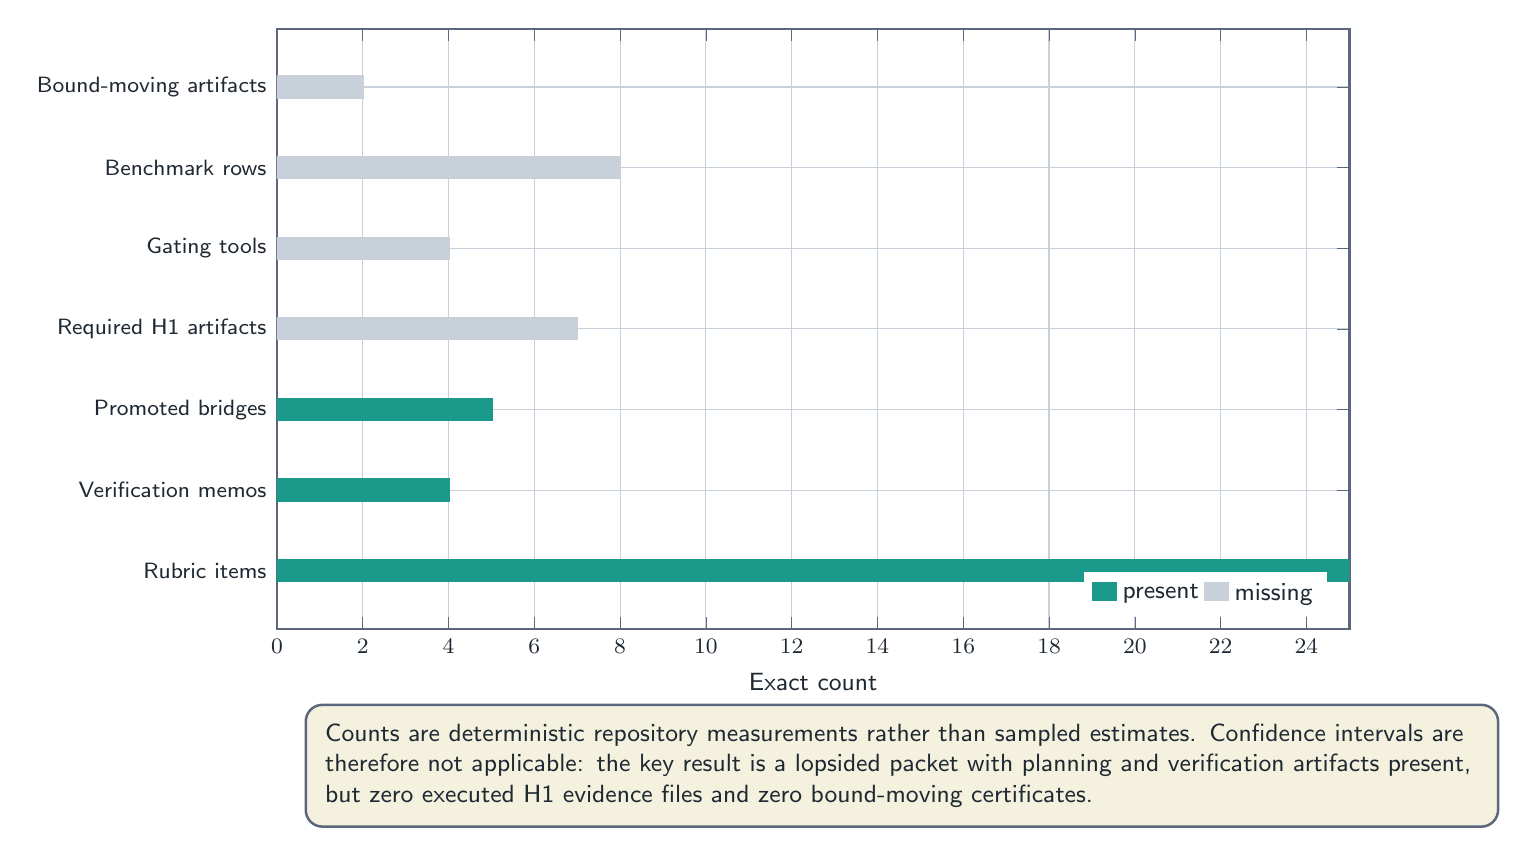
\begin{tikzpicture}
  \begin{axis}[
    xbar stacked,
    width=15.2cm,
    height=9.2cm,
    xmin=0,
    xmax=25,
    grid=major,
    bar width=7.5pt,
    xlabel={Exact count},
    symbolic y coords={
      Bound-moving artifacts,
      Benchmark rows,
      Gating tools,
      Required H1 artifacts,
      Promoted bridges,
      Verification memos,
      Rubric items
    },
    ytick=data,
    y dir=reverse,
    enlarge y limits=0.12,
    legend columns=2,
    legend style={at={(0.98,0.02)},anchor=south east}
  ]
    \addplot+[xbar, fill=archTeal, draw=archTeal] coordinates {
      (0,Bound-moving artifacts)
      (0,Benchmark rows)
      (0,Gating tools)
      (0,Required H1 artifacts)
      (5,Promoted bridges)
      (4,Verification memos)
      (25,Rubric items)
    };
    \addplot+[xbar, fill=archStone, draw=archStone] coordinates {
      (2,Bound-moving artifacts)
      (8,Benchmark rows)
      (4,Gating tools)
      (7,Required H1 artifacts)
      (0,Promoted bridges)
      (0,Verification memos)
      (0,Rubric items)
    };
    \legend{present, missing}
  \end{axis}

  \node[note, text width=14.65cm, anchor=north west] at (0.35,-0.95) {
    Counts are deterministic repository measurements rather than sampled estimates.
    Confidence intervals are therefore not applicable: the key result is a lopsided packet with
    planning and verification artifacts present, but zero executed H1 evidence files and zero
    bound-moving certificates.
  };
\end{tikzpicture}
\end{document}
